\pdfminorversion=4
\documentclass[aspectratio=169]{beamer}

\mode<presentation>
{
  \usetheme{default}
  \usecolortheme{default}
  \usefonttheme{default}
  \setbeamertemplate{navigation symbols}{}
  \setbeamertemplate{caption}[numbered]
  \setbeamertemplate{footline}[frame number]  % or "page number"
  \setbeamercolor{frametitle}{fg=white}
  \setbeamercolor{footline}{fg=black}
} 

\usepackage[english]{babel}
\usepackage[utf8x]{inputenc}
\usepackage{tikz}
\usepackage{courier}
\usepackage{array}
\usepackage{bold-extra}
\usepackage{minted}
\usepackage[thicklines]{cancel}
\usepackage{fancyvrb}

\xdefinecolor{dianablue}{rgb}{0.18,0.24,0.31}
\xdefinecolor{darkblue}{rgb}{0.1,0.1,0.7}
\xdefinecolor{darkgreen}{rgb}{0,0.5,0}
\xdefinecolor{darkgrey}{rgb}{0.35,0.35,0.35}
\xdefinecolor{darkorange}{rgb}{0.8,0.5,0}
\xdefinecolor{darkred}{rgb}{0.7,0,0}
\definecolor{darkgreen}{rgb}{0,0.6,0}
\definecolor{mauve}{rgb}{0.58,0,0.82}

\title[2020-11-20-cms-analysistools-workshop]{Survey and status of Pythonic HEP analysis tools}
\author{Jim Pivarski}
\institute{Princeton University -- IRIS-HEP}
\date{November 20, 2020}

\usetikzlibrary{shapes.callouts}

\begin{document}

\logo{\pgfputat{\pgfxy(0.11, 7.4)}{\pgfbox[right,base]{\tikz{\filldraw[fill=dianablue, draw=none] (0 cm, 0 cm) rectangle (50 cm, 1 cm);}\mbox{\hspace{-8 cm}
\includegraphics[height=1 cm]{princeton-logo-long.png}\hspace{0.1 cm}\raisebox{0.1 cm}{
\includegraphics[height=0.8 cm]{iris-hep-logo-long.png}}\hspace{0.1 cm}}}}}

\begin{frame}
  \titlepage
\end{frame}

\logo{\pgfputat{\pgfxy(0.11, 7.4)}{\pgfbox[right,base]{\tikz{\filldraw[fill=dianablue, draw=none] (0 cm, 0 cm) rectangle (50 cm, 1 cm);}\mbox{\hspace{-8 cm}
\includegraphics[height=1 cm]{princeton-logo.png}\hspace{0.1 cm}\raisebox{0.1 cm}{
\includegraphics[height=0.8 cm]{iris-hep-logo.png}}\hspace{0.1 cm}}}}}

% Uncomment these lines for an automatically generated outline.
%\begin{frame}{Outline}
%  \tableofcontents
%\end{frame}

% START START START START START START START START START START START START START

\begin{frame}{Needless to say, CMS is already using Python a lot!}
\vspace{0.5 cm}
\only<1>{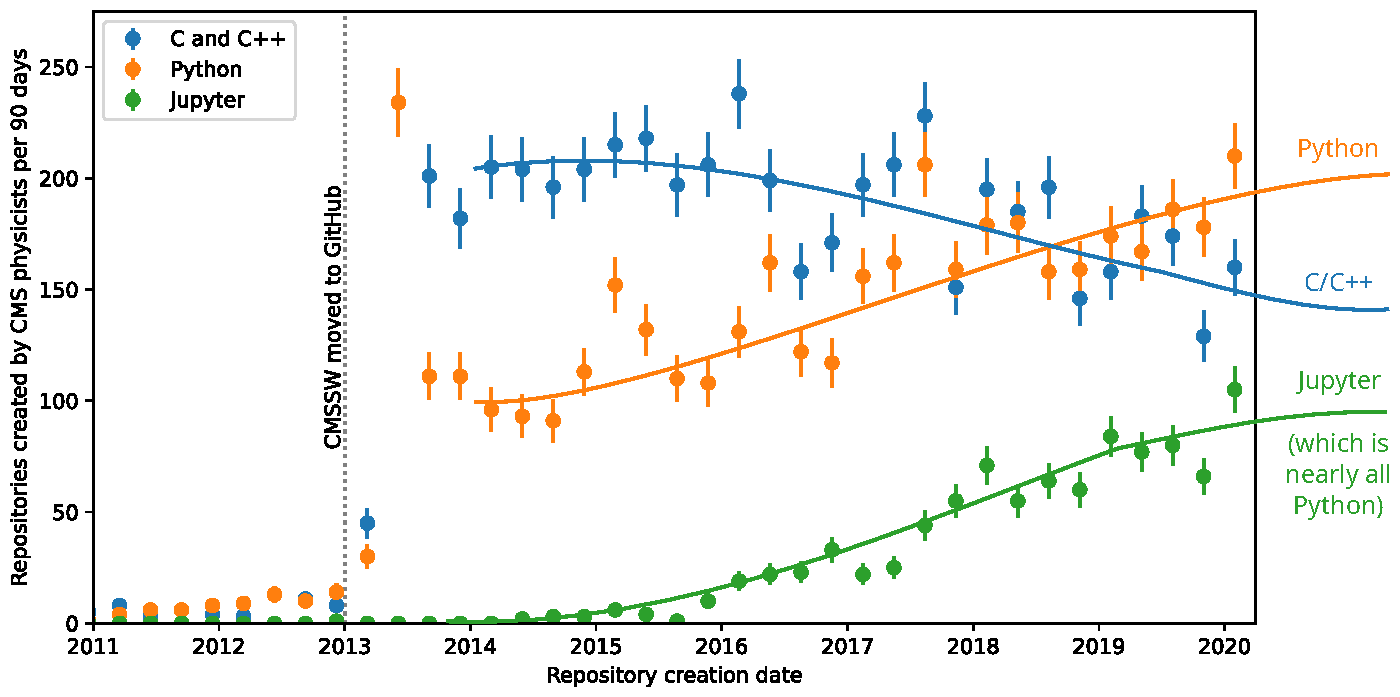
\includegraphics[width=\linewidth]{01-github-cmssw-language.pdf}}\only<2>{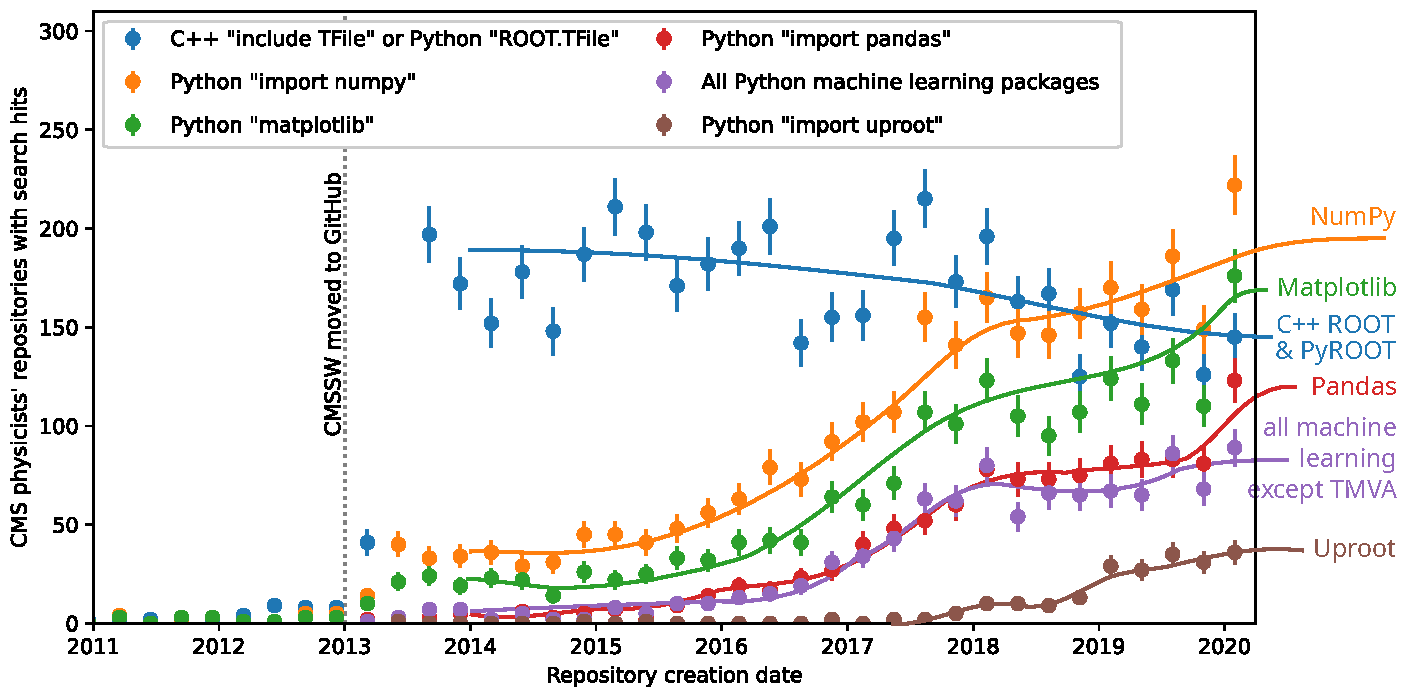
\includegraphics[width=\linewidth]{05-github-anyroot-python-machinelearning-uproot.pdf}}
\end{frame}

\begin{frame}{But I'll be talking about the Scikit-HEP tools}
\large

\vspace{0.2 cm}
\hfill 
\includegraphics[height=3 cm]{scikit-hep-logo.pdf}

\vspace{-2 cm}
\begin{itemize}\setlength{\itemsep}{0.2 cm}
\item<1-> Experiment agnostic
\item<2-> Connects to industry-standard ecosystem (NumPy, etc.)
\item<3-> Provides capabilities that don't exist in the larger ecosystem

\vspace{0.2 cm}
\begin{itemize}\setlength{\itemsep}{0.2 cm}
\item<4-> \normalsize because it's domain-specific: e.g.\ Lorentz vectors
\item<5-> \normalsize because HEP is a pioneer: e.g.\ histograms-as-objects
\end{itemize}

\vspace{0 cm}
\item<6-> Technical: focuses on columnar data to mitigate Python's speed issue

\begin{uncoverenv}<6->
\begin{center}
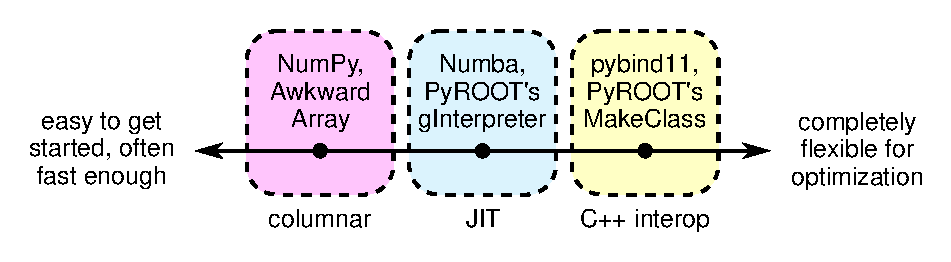
\includegraphics[width=0.75\linewidth]{ease-vs-flexibility.pdf} \mbox{\hspace{1 cm}}
\end{center}
\end{uncoverenv}
\end{itemize}
\end{frame}

\begin{frame}{This is a survey talk}
\vspace{0.17 cm}
\begin{columns}
\column{1.15\linewidth}
\only<1>{
\includegraphics[width=\linewidth]{survey-1.pdf}}\only<2>{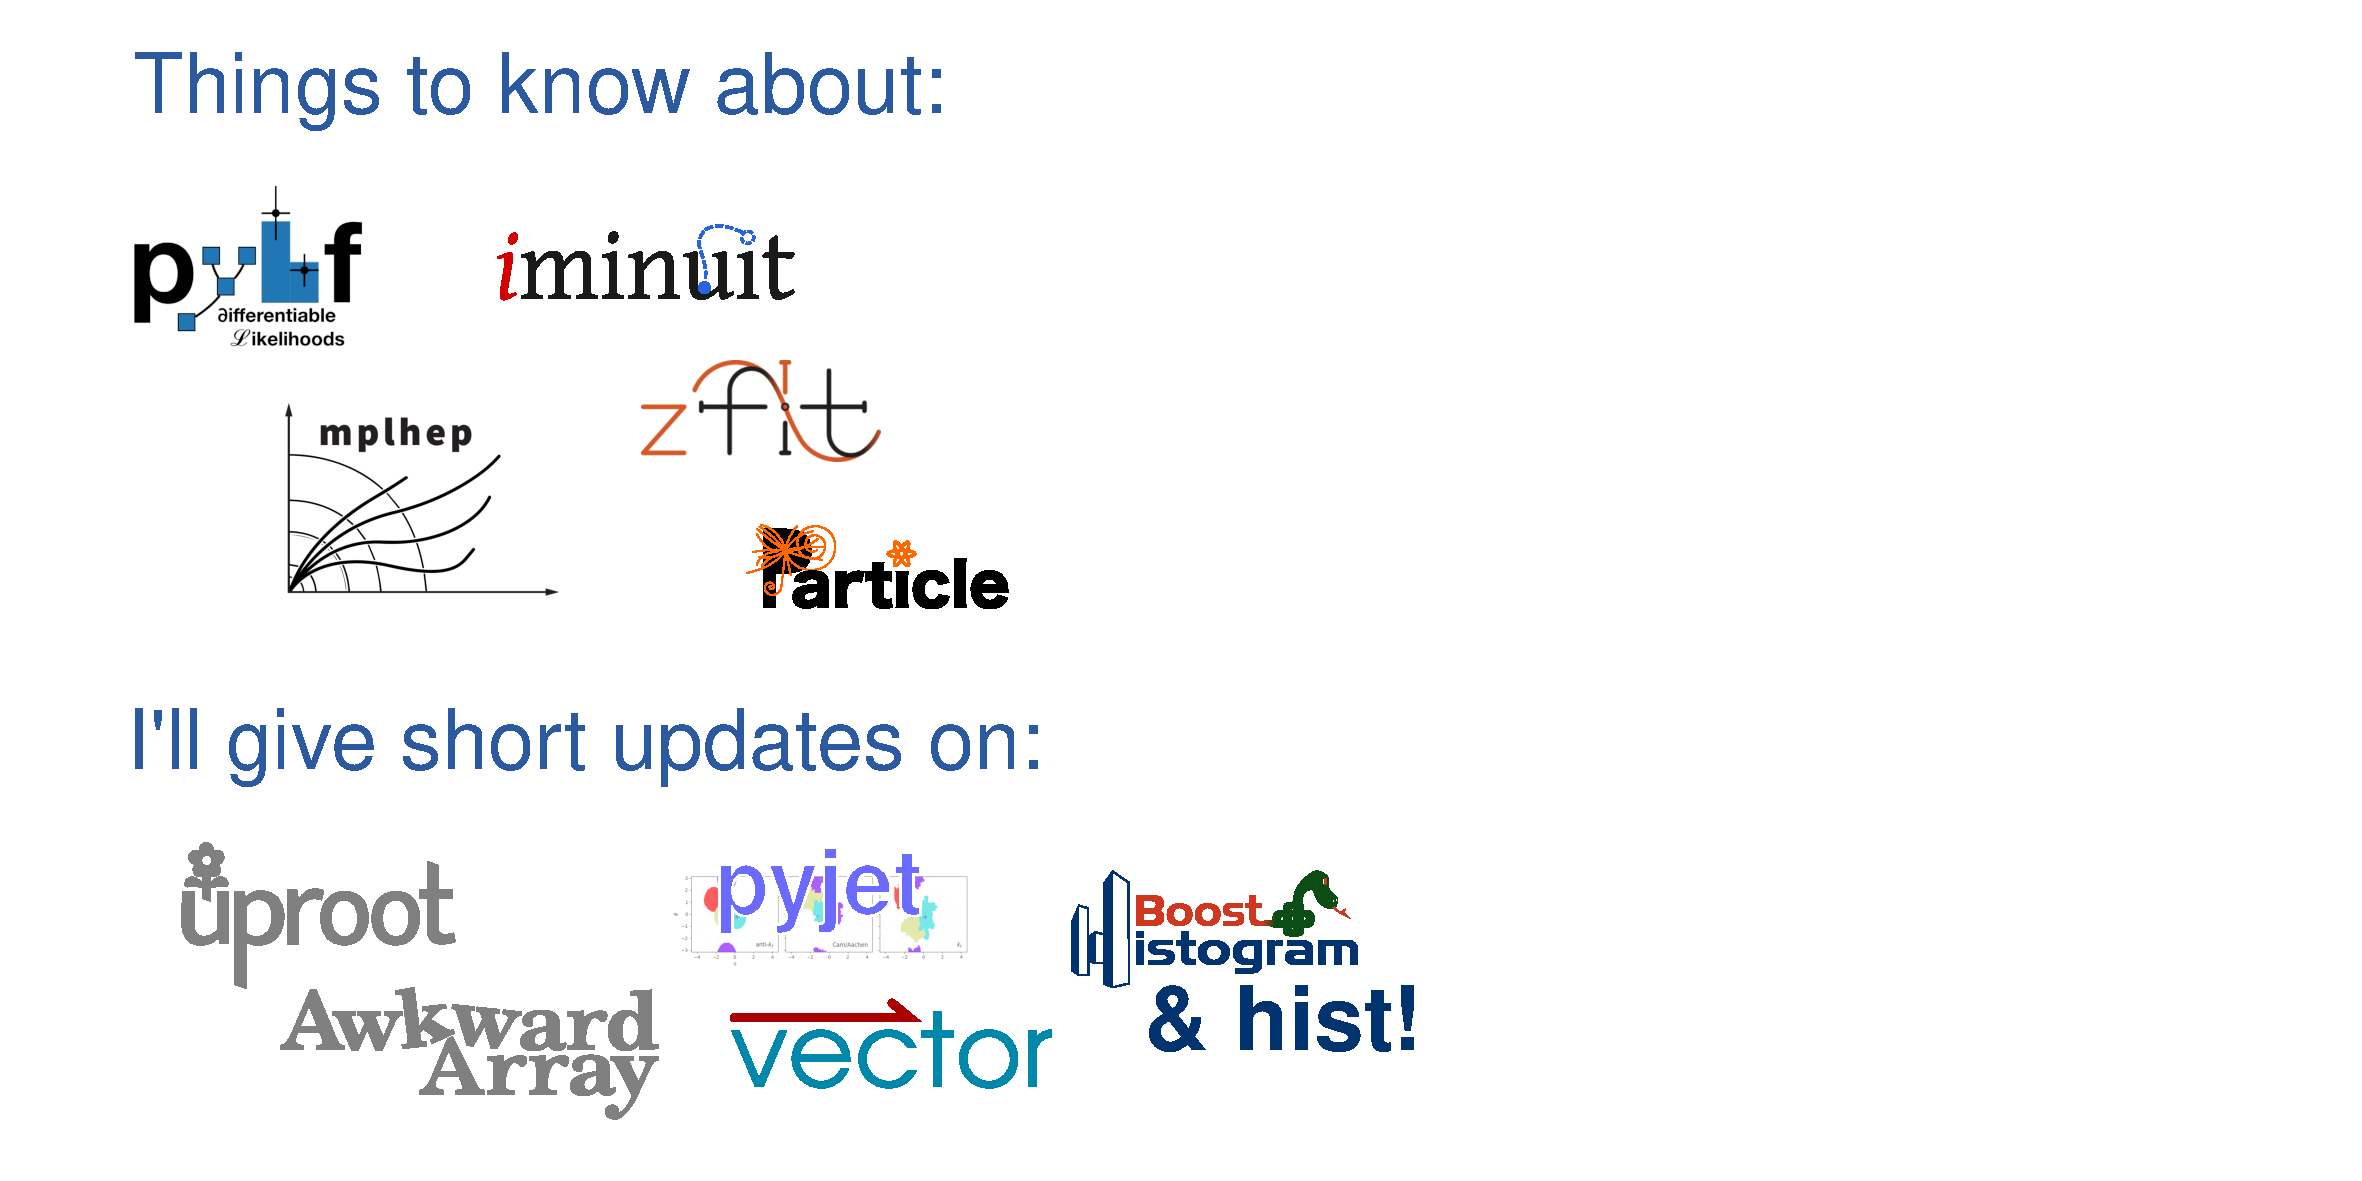
\includegraphics[width=\linewidth]{survey-2.pdf}}\only<3>{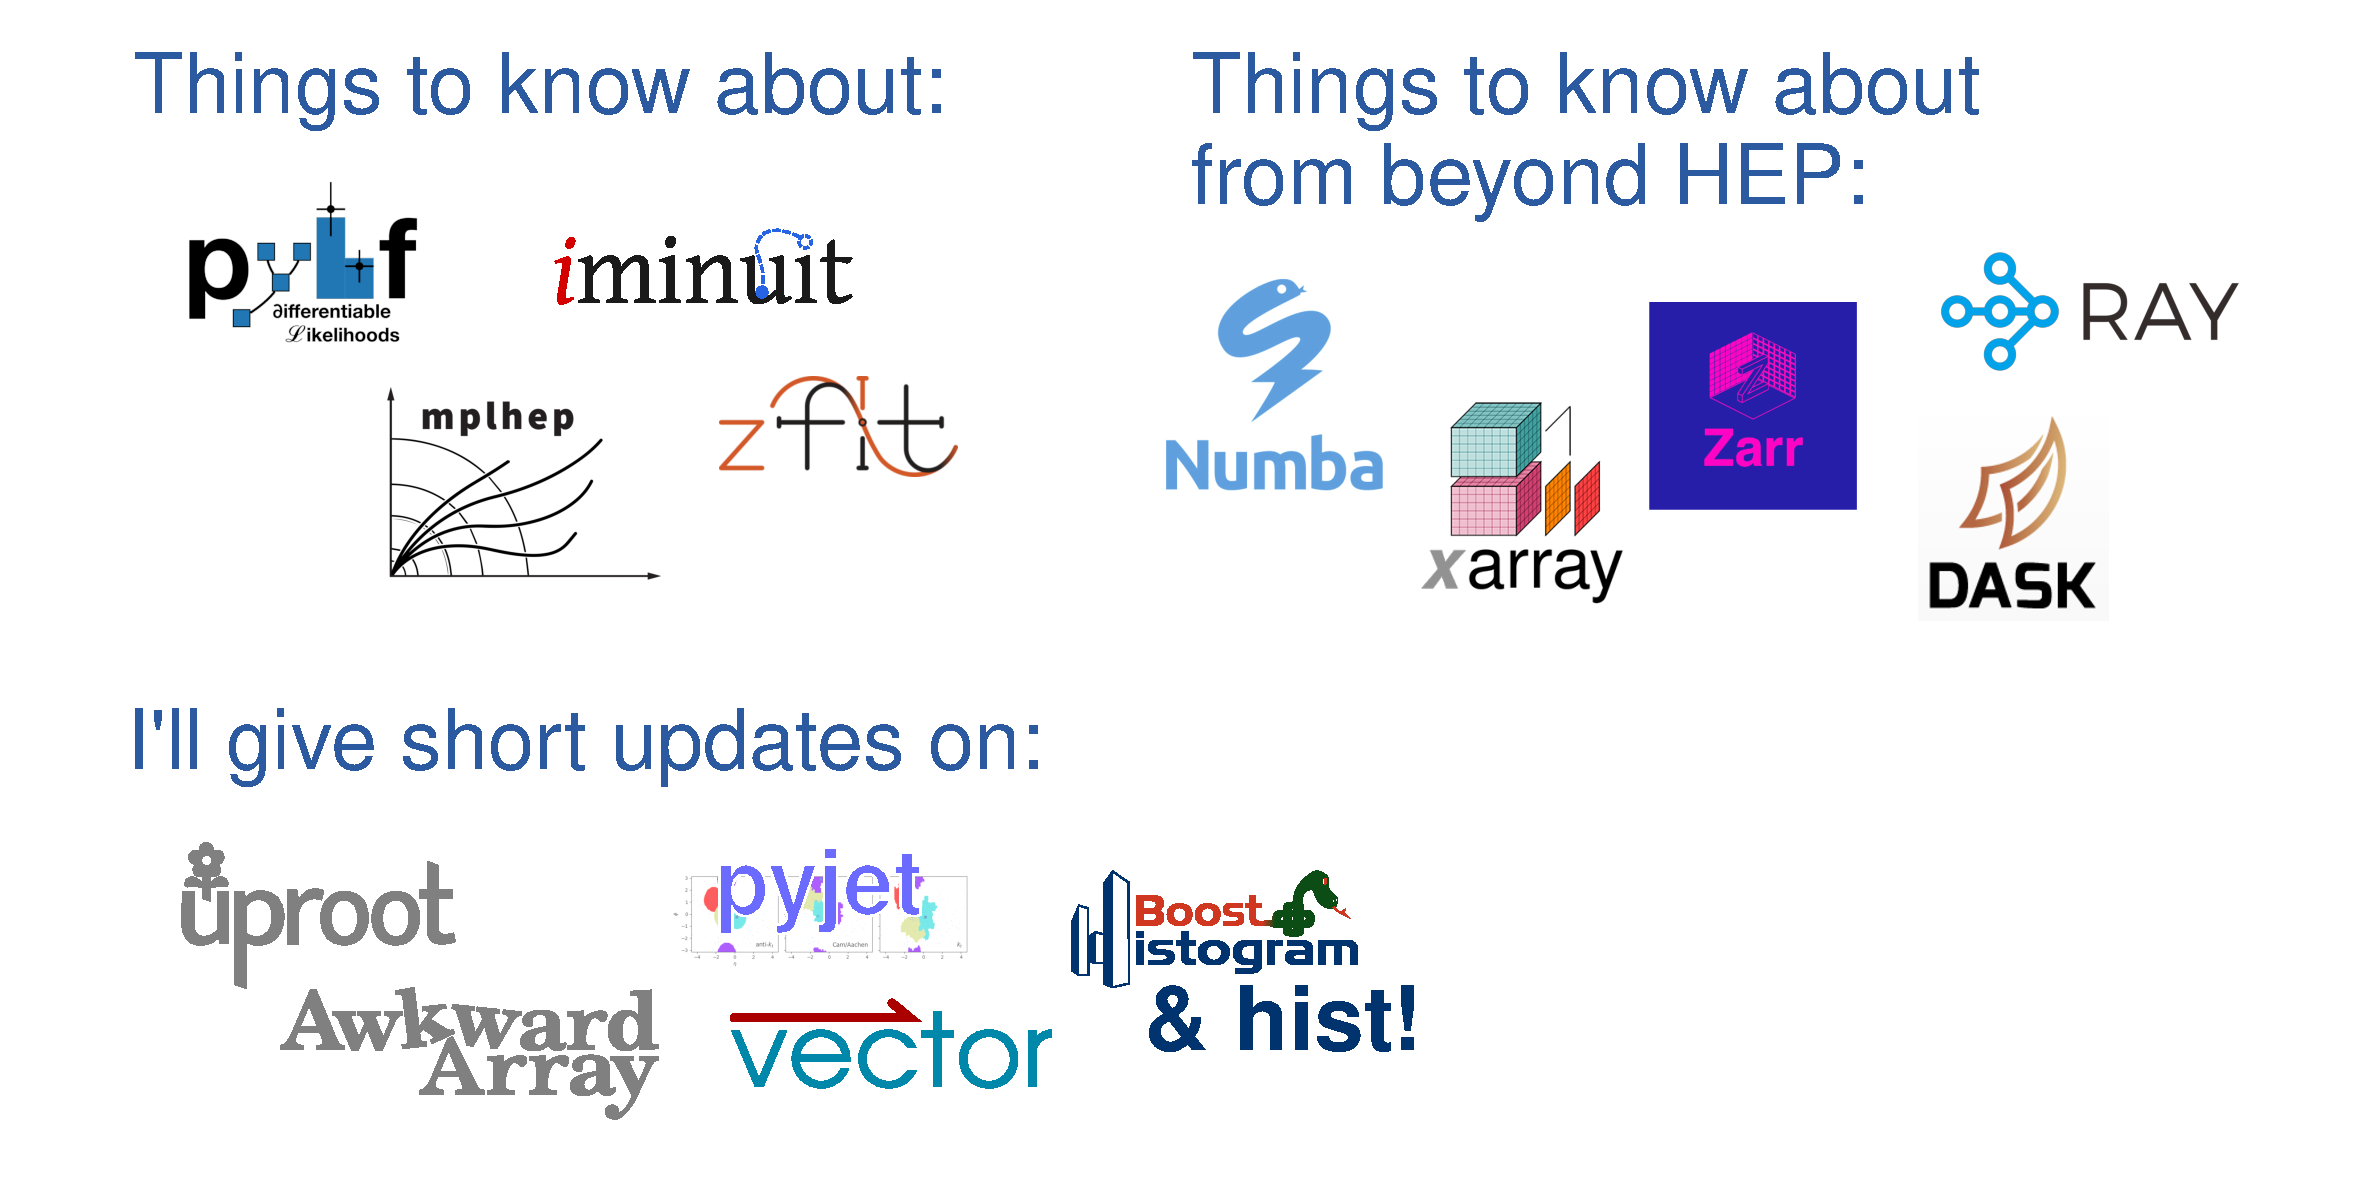
\includegraphics[width=\linewidth]{survey-3.pdf}}\only<4>{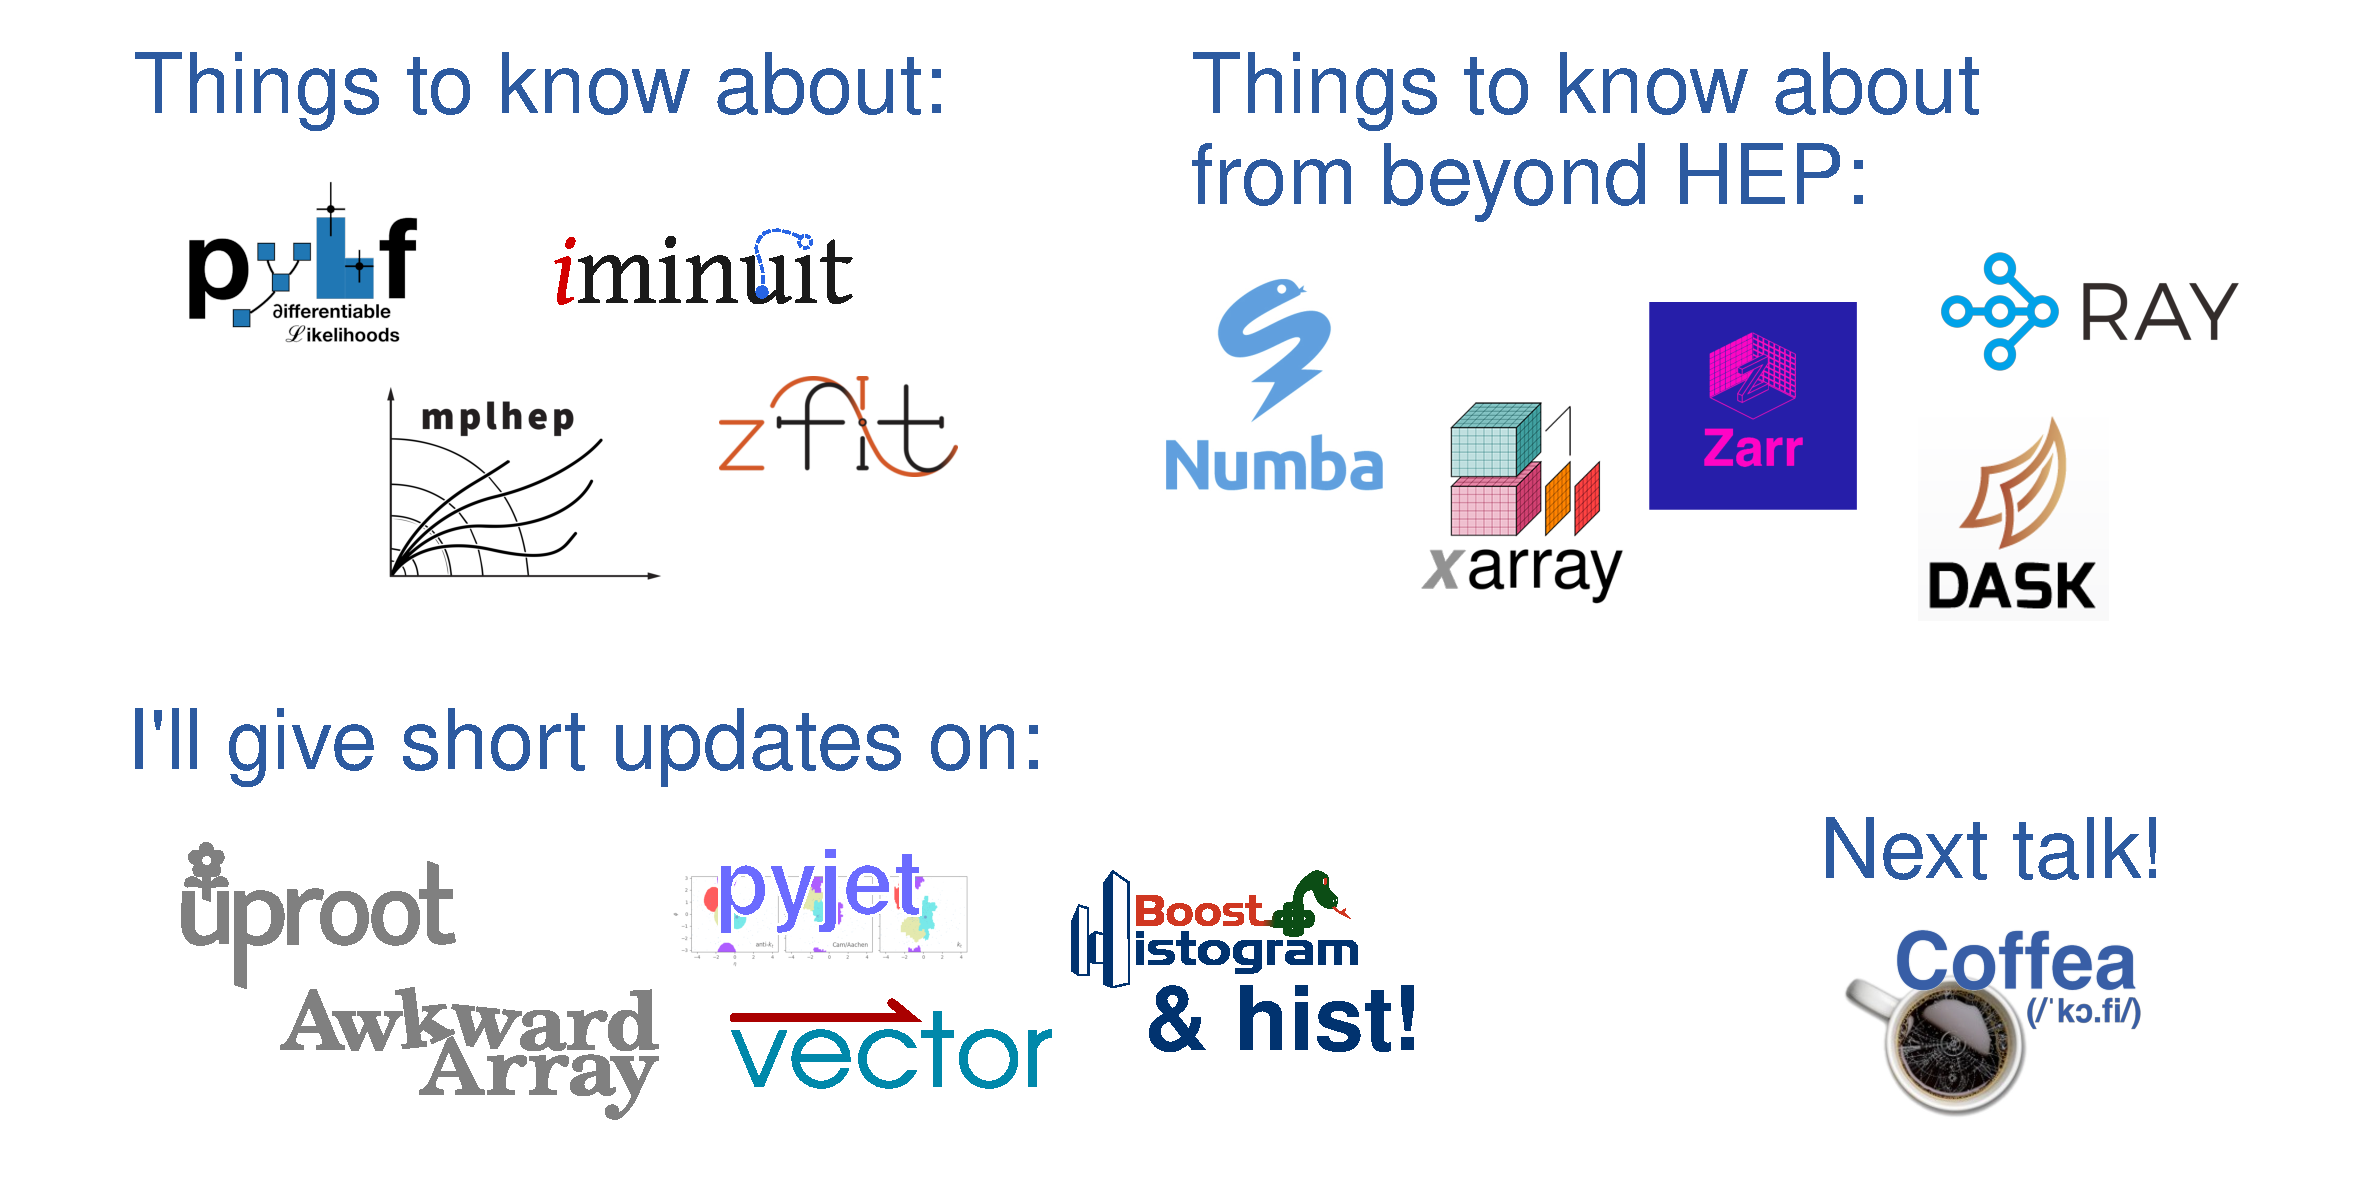
\includegraphics[width=\linewidth]{survey-4.pdf}}
\end{columns}
\end{frame}




\end{document}
